\makeheading{Week 12}
\section{Response Surface Experiments}
\begin{itemize}
    \item[*] Effective experimentation is sequential: information gained in one experiment can help to inform future
        experiments.
    \item Screening experiments are used to identify which among numerous factors are the ones that
          significantly influence the response variable.
    \item We follow these up with further experimentation where the goal is \textbf{response optimization}.
          \begin{itemize}
              \item \textbf{Method of Steepest Ascent/Descent}.
              \item \textbf{Response Surface Designs}.
          \end{itemize}
    \item In these investigations, response optimization requires investigating and characterizing response surfaces of the form:
          \[ \E{Y}=f(x_1,x_2,\ldots,x_{K^\prime}) \]
          (for a continuous response) and
          \[ \log*{\frac{\E{Y}}{1-\E{Y}}}=f(x_1,x_2,\ldots,x_{K^\prime}) \]
          (for a binary response).
\end{itemize}
\subsection*{Finding the Optimum}
\begin{itemize}
    \item Supposing that sufficient data is collected and the second-order model may be fitted, we obtain the
          estimated response surface.
          \[ \hat{\eta}=\hat{\beta}_0+\sum_{j=1}^{K^\prime} \hat{\beta}_j x_j+\sum_{j<\ell}\hat{\beta}_{j\ell}x_j x_\ell +\sum_{j=1}^{K^\prime} \hat{\beta}_{jj}x_j^2  \]
    \item This expression may be re-written in vector-matrix notation as:
          \[ \hat{\eta}=\hat{\beta}_0+\Vector{x}^\top \Vector{b}+\Vector{x}^\top\Matrix{B}\Vector{x} \]
          where
          \[ \Vector{x}=\begin{bmatrix}
                  x_1    \\
                  x_2    \\
                  \vdots \\
                  x_{K^\prime}
              \end{bmatrix},\qquad
              \Vector{b}=\begin{bmatrix}
                  \hat{\beta}_1 \\
                  \hat{\beta}_2 \\
                  \vdots        \\
                  \hat{\beta}_{K^\prime}
              \end{bmatrix},\qquad
              \Matrix{B}=\begin{bmatrix}
                  \hat{\beta}_{11}                   & \frac{1}{2}\hat{\beta}_{12}        & \cdots & \frac{1}{2}\hat{\beta}_{1K^\prime} \\
                  \frac{1}{2}\hat{\beta}_{12}        & \hat{\beta}_{22}                   & \cdots & \frac{1}{2}\hat{\beta}_{2K^\prime} \\
                  \vdots                             & \vdots                             & \ddots & \vdots                             \\
                  \frac{1}{2}\hat{\beta}_{1K^\prime} & \frac{1}{2}\hat{\beta}_{2K^\prime} & \cdots & \hat{\beta}_{K^\prime K^\prime}
              \end{bmatrix} \]
          \begin{itemize}
              \item $ \Vector{x} $ is a $ K^\prime \times 1 $ vector of specific factor values.
              \item $ \Vector{b} $ is a $ K^\prime \times 1 $ vector of the estimates of the main effect coefficients.
              \item $ \Matrix{B} $ is a $ K^\prime \times K^\prime $ symmetric matrix of second-order effect estimates
                    (i.e., the second-order interactions and quadratic effects).
          \end{itemize}
    \item In order to find the value of $ \Vector{x}=(x_1,x_2,\ldots,x_{K^\prime})^\top $ that maximizes/minimizes the expected response,
          we must find the \textbf{stationary point} of the estimated response surface.
    \item The stationary point is:
          \[ \Vector{x}_{\symbfsfup{s}}=-\frac{1}{2} \Matrix{B}^{-1}\Vector{b} \]
          which is found by solving:
          \[ \pdv{\hat{\eta}}{\Vector{x}}=\Vector{b}+2\Matrix{B}\Vector{x}=\Vector{0} \]
    \item The optimal expected response is:
          \[ \widehat{\E{Y}}=\hat{\eta}_{\symbfsfup{s}}=\hat{\beta}_0+\frac{1}{2} \Vector{x}^\top_{\symbfsfup{s}} \Vector{b} \]
          in the case of linear regression and
          \[ \widehat{\E{Y}}=\frac{\exp{\hat{\eta}_{\symbfsfup{s}}}}{1+\exp{\hat{\eta}_{\symbfsfup{s}}}}
              =\frac{\exp{\hat{\beta}_0+\frac{1}{2} \Vector{x}^\top_{\symbfsfup{s}} \Vector{b}}}{1+\exp{\hat{\beta}_0+\frac{1}{2} \Vector{x}^\top_{\symbfsfup{s}} \Vector{b}}} \]
          in the case of logistic regression.
    \item For practical implementation of this solution, the stationary point $ \Vector{x}_{\symbfsfup{s}} $ must be translated into optimal
          operating conditions in natural units $ \Vector{U}_{\symbfsfup{s}} $ using the following conversion formula:
          \[ U=x\times \frac{U_{\symbfsfup{H}}-U_{\symbfsfup{L}}}{2}+\frac{U_{\symbfsfup{H}}+U_{\symbfsfup{L}}}{2}  \]
    \item[*] However, for us to be confident that $ \Vector{x}_{\symbfsfup{s}} $ indeed optimizes $ f(\:\cdot\:) $, we must be confident that $ \eta $ and, in particular,
        that $ \hat{\eta} $ adequately represents $ f(\:\cdot\:) $.
        \begin{itemize}
            \item[*] Since we only expect the second-order approximation to be adequate in a small localized region,
                it is important that this small localized region contains the true optimum.
            \item It is quite unlikely that the values of $ x_1,x_2,\ldots,x_{K^\prime} $ considered in the screening phase are close
                  to the optimum.
            \item[*] This is why we needed the method of steepest ascent/descent.
                \begin{itemize}
                    \item[*] This intermediate phase of experimentation helped us determine roughly where the region of
                        the optimum lies.
                \end{itemize}
        \end{itemize}
\end{itemize}
\subsection{The Central Composite Design}
\begin{itemize}
    \item[*] The goal of a response surface experiment is to be able to fit a full second-order response surface model.
        \begin{itemize}
            \item This requires estimating $ (K^\prime+1)(K^\prime+2)/2 $ coefficients.
        \end{itemize}
    \item Several such designs exist (i.e., ``response surface''), but here we study one in particular: the \textbf{central composite design} (CCD).
    \item A CCD is typified by three different types of experimental conditions:
          \begin{enumerate}[i.]
              \item \textbf{two-level} factorial conditions,
              \item a \textbf{centre point} condition, and
              \item \textbf{axial}, or \emph{star}, conditions.
          \end{enumerate}
    \item In other words,
          \begin{enumerate}[i.]
              \item The factorial conditions constitute a full $ 2^{K^\prime} $ factorial design.
              \item The centre point condition sits at $ x_1=x_2=\cdots=x_{K^\prime}=0 $ in the centre of the factorial ones.
              \item The axial conditions sit `outside' of the factorial ones at $ \pm a $ on each of the $ K^\prime $ factors' axes. Note that $ a $ is defined in coded units.
          \end{enumerate}
    \item When investigating $ K^\prime $ factors the central composite design therefore requires $ 2^{K^\prime}+2K^\prime+1 $ distinct experimental conditions.
    \item These designs may be visualized geometrically as we see in the figures below, for $ K^\prime=1,2,3 $.
    \item The design matrices that give rise to these designs (for $ K^\prime=1,2,3 $) are shown in~\Cref{tab:exampledesigns}.
          \begin{table}[!htbp]
              \centering
              \caption{Design matrices associated with central composite designs on $ K^\prime=1 $ (left), $ K^\prime=2 $ (middle) and $ K^\prime=3 $ (right) factors.}\label{tab:exampledesigns}
              \begin{tabular}{cc}
                  \toprule Condition & $x_{1}$ \\
                  \midrule 1         & $-1$    \\
                  2                  & $+1$    \\
                  3                  & $-a$    \\
                  4                  & $+a$    \\
                  5                  & 0       \\
                  \bottomrule
              \end{tabular}\hfill
              \begin{tabular}{ccc}
                  \toprule Condition & $x_{1}$ & $x_{2}$ \\
                  \midrule 1         & $-1$    & $-1$    \\
                  2                  & $+1$    & $-1$    \\
                  3                  & $-1$    & $+1$    \\
                  4                  & $+1$    & $+1$    \\
                  5                  & $-a$    & 0       \\
                  6                  & $+a$    & 0       \\
                  7                  & 0       & $-a$    \\
                  8                  & 0       & $+a$    \\
                  9                  & 0       & 0       \\
                  \bottomrule
              \end{tabular}\hfill
              \begin{tabular}{cccc}
                  \toprule Condition & $x_{1}$ & $x_{2}$ & $x_{3}$ \\
                  \midrule 1         & $-1$    & $-1$    & $-1$    \\
                  2                  & $+1$    & $-1$    & $-1$    \\
                  3                  & $-1$    & $+1$    & $-1$    \\
                  4                  & $+1$    & $+1$    & $-1$    \\
                  5                  & $-1$    & $-1$    & $+1$    \\
                  6                  & $+1$    & $-1$    & $+1$    \\
                  7                  & $-1$    & $+1$    & $+1$    \\
                  8                  & $+1$    & $+1$    & $+1$    \\
                  9                  & $-a$    & 0       & 0       \\
                  10                 & $+a$    & 0       & 0       \\
                  11                 & 0       & $-a$    & 0       \\
                  12                 & 0       & $+a$    & 0       \\
                  13                 & 0       & 0       & $-a$    \\
                  14                 & 0       & 0       & $+a$    \\
                  15                 & 0       & 0       & 0       \\
                  \bottomrule
              \end{tabular}
          \end{table}
    \item \textbf{Choosing} $ a $:
          \begin{itemize}
              \item The value of $ a $ is determined by the experimenter, and may be chosen to balance both practical
                    and statistical concerns.
              \item The experimenter must be mindful of the constraints imposed by the region of operability and
                    whether the natural-unit counterpart to $ a $ is something inconvenient/infeasible.
              \item Barring practical constraints, two common choices for $ a $ are $ a=1 $ and $ a=\sqrt{K^\prime} $.
          \end{itemize}
    \item $ a=1 $:
          \begin{itemize}
              \item The CCD reduces to a $ 3^{K^\prime} $ design.
              \item It is referred to as \emph{face-centred central composite design}.
              \item A benefit is that it requires just 3 (not 5) levels for every factor.
              \item Another benefit is that it is a cuboidal design and so it inherits some usual conveniences
                    associated with orthogonal cuboidal designs.
              \item You might choose $ a=1 $ if the region of the optimum is in a corner of the region of operability, and hence $ a=1 $ keeps the experimental conditions inside the
                    region of operability.
          \end{itemize}
    \item $ a=\sqrt{K^\prime} $:
          \begin{itemize}
              \item In this design the axial conditions are at an equal distance from the centre point as the factorial
                    conditions.
              \item Such a design is referred to as \emph{spherical} since it places all axial and factorial conditions on a ``hyper'' sphere of radius $ \sqrt{K^\prime} $.
              \item The benefit of such equal spacing is that it ensures that the estimate of the response surface at each condition is equally precise.
                    \begin{itemize}[$\hookrightarrow$]
                        \item Designs with this property are called \underline{rotatable}.
                    \end{itemize}
          \end{itemize}
    \item[*] No matter the choice of $ a>0 $, the CCD facilitates estimation of the full second-order response surface
        model, and hence identification of the optimum.
\end{itemize}
\subsection{The Lyft Example}
\begin{itemize}
    \item We illustrate the design and analysis of a central composite experiment in the context of a common
          ride-sharing problem.
    \item Suppose that Lyft is interested in designing a promotional offer that maximizes ride-bookings during
          an experimental period.
    \item[$\rightarrow$] Previous screening experiments evaluated the influence of discount amount, discount duration, ride
        type, time-of-day, and the method of dissemination. It was found that the most important factors
        were discount amount ($ x_1 $) and discount duration ($ x_2 $).
    \item A previous steepest ascent exercise also suggested that the optimal discount duration is somewhere in
          the vicinity of \qty{4.5}{\day} and the optimal discount amount is somewhere in the vicinity of \qty{50}{\percent}.
    \item To find optimal values of these factors a follow-up two-factor central composite design was run in order
          to fit a second-order response surface model.
    \item The experimental conditions (in both coded and natural units) are shown in~\Cref{tab:Lyft}.
          \begin{table}[!htbp]
              \centering
              \caption{Booking rate by condition in the Lyft experiment.}\label{tab:Lyft}
              \begin{tabular}{
                      S[table-format=1]
                      S[table-format=2]
                      S[table-format=-1.2]
                      S[table-format=1.1]
                      S[table-format=-1.2]
                      S[table-format=1.2]
                  }
                  \toprule {Condition} & {Discount Amount (\unit{\percent})} & {$x_{1}$} & {Discount Duration (\unit{\day})} & {$x_{2}$} & {Booking Rate} \\
                  \midrule
                  1                    & 25                                  & -1        & 2                                 & -1        & 0.71           \\
                  2                    & 75                                  & +1        & 2                                 & -1        & 0.32           \\
                  3                    & 25                                  & -1        & 7                                 & +1        & 0.71           \\
                  4                    & 75                                  & +1        & 7                                 & +1        & 0.35           \\
                  5                    & 85                                  & +1.4      & 4.5                               & 0         & 0.53           \\
                  6                    & 15                                  & -1.4      & 4.5                               & 0         & 0.50           \\
                  7                    & 50                                  & 0         & 8                                 & +1.4      & 0.26           \\
                  8                    & 50                                  & 0         & 1                                 & -1.4      & 0.78           \\
                  9                    & 50                                  & 0         & 4.5                               & 0         & 0.72           \\
                  \bottomrule
              \end{tabular}
          \end{table}
    \item \textbf{NOTE}: that the experimenters had intended to perform axial conditions with $ a=\sqrt{2} $, but the
          corresponding discount amounts and discount durations were:
          \[ (\qty{14.64466}{\percent},\qty{85.35534}{\percent})\text{ and } (\qty{0.9644661}{\day}, \qty{8.035534}{\day}) \]
          In the interest of defining experimental conditions with practically convenient
          levels they opted for $ a = 1.4 $ yielding the discount amounts and durations shown in~\Cref{tab:Lyft}.
    \item $ n = 500 $ users were then randomized into each of these $ m = 9 $ conditions and for each user, whether
          they booked a ride in the experimentation period was recorded.
          \begin{itemize}
              \item The booking rates in each condition are also shown in~\Cref{tab:Lyft}.
          \end{itemize}
    \item The output from the fitted second-order logistic regression model is shown in~\Cref{tab:lyftOUT}.
          \begin{table}[!htbp]
              \centering
              \caption{Summary of second-order logistic regression model.}\label{tab:lyftOUT}
              \begin{tabular}{c
                      S[table-format=-1.3]
                      S[table-format=1.3]
                      S[table-format=-2.3]
                      S[table-format=<1.3e-2]}
                  \toprule
                                      & {Estimate}              & {Std. Error}           & {$ t $-value}           & {$ \Pr({>\abs{t}}) $} \\
                  \midrule
                  (Intercept)         & 0.94284495807779089560  & 0.09952415473335386731 & 9.4735300000000002285   & < 2.222e-16           \\
                  $x_1$               & 0.03880948377397467480  & 0.03306830373987898475 & 1.1736200000000001076   & 2.4055e-01            \\
                  $x_2$               & -0.80683569762176121642 & 0.03568166276802093445 & -22.6120499999999999829 & < 2.222e-16           \\
                  $\mathrm{I}(x_1^2)$ & -0.44206629932557028884 & 0.05788383995433134255 & -7.6371299999999999741  & 2.2212e-14            \\
                  $\mathrm{I}(x_2^2)$ & -0.41447782996612042572 & 0.05930513400228028947 & -6.9889000000000001123  & 2.7704e-12            \\
                  $x_1\text{:}x_2$    & 0.03391918751995325748  & 0.04846198700619906014 & 0.6999100000000000321   & 4.8398e-01            \\
                  \bottomrule
              \end{tabular}
          \end{table}
    \item Contour plots of the fitted response surface are shown in~\Cref{fig:Lyft}.
          \begin{figure}[!htbp]
              \centering
              \begin{subfigure}{0.48\textwidth}
                  \centering
                  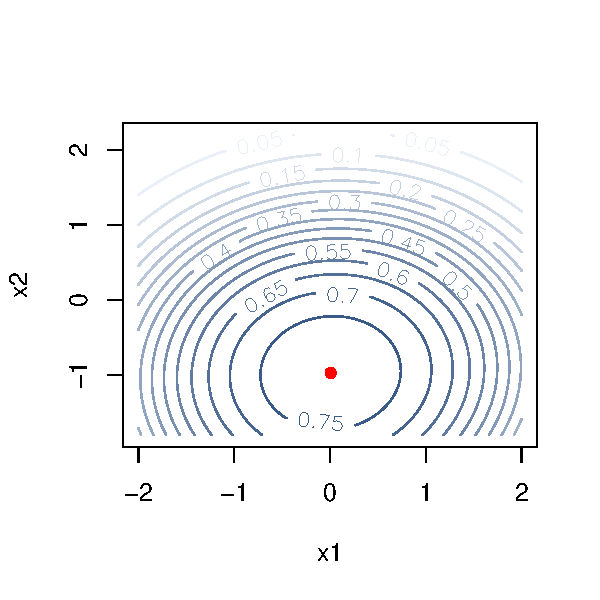
\includegraphics[width=\linewidth]{lyft1.pdf}\caption{}\label{subfig:Lyft1}
              \end{subfigure}
              \begin{subfigure}{0.48\textwidth}
                  \centering
                  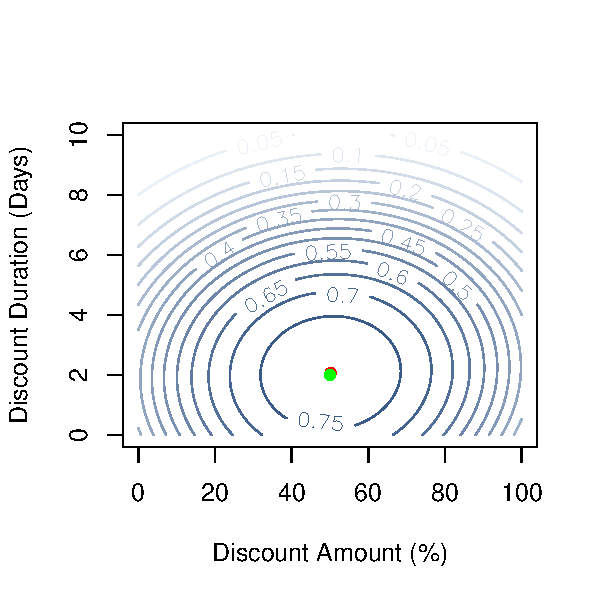
\includegraphics[width=\linewidth]{lyft2.pdf}\caption{}\label{subfig:Lyft2}
              \end{subfigure}
              \caption{2D contour plots of the second-order Lyft model.
                  \Cref{subfig:Lyft1}: Coded-Unit Factor Space.
                  \Cref{subfig:Lyft2}: Natural-Unit Factor Space.}\label{fig:Lyft}
          \end{figure}
    \item The stationary point for this second-order model is located (in coded units) at $ x_1 = \num{0.006565206}$,
          $ x_2 = \num{-0.973047233} $ using $ \Vector{x}_{\symbfsfup{s}}=-\frac{1}{2} \Matrix{B}^{-1}\Vector{b} $.
          \begin{itemize}
              \item In the natural units this corresponds to a discount rate of \qty{50.16413}{\percent} that lasts for \qty{2.067382}{\day}.
              \item The predicted booking rate at this point is \num{0.7917517}, with a \qty{95}{\percent} prediction interval given by
                    $(\num{0.769111734827683}, \num{0.81439175121308})$.
          \end{itemize}
    \item A slightly less optimal but more practically feasible promotion would be a
          \qty{50}{\percent} discount lasting \qty{2}{\day} (this is what Lyft should move forward with into a \underline{confirmation} phase).
          \begin{itemize}
              \item This achieves a booking rate of \num{0.791699940932622} with a \qty{95}{\percent} prediction interval of
                    $(\num{0.769265741331575}, \num{0.81413414053367})$.
          \end{itemize}
    \item \href{https://github.com/Hextical/university-notes/blob/master/year-3/semester-3/STAT 430/code/W12/CCD_example.R}{[R Code] \texttt{CCD\_example}}
\end{itemize}
\section{RSM with Qualitative Factors}
\begin{itemize}
    \item What do you do if you have $ \ge 1 $ categorical factors in addition to our numeric factor(s)?
    \item[*] Everything that has been discussed thus far with respect to central composite designs and response
        surface optimization has assumed that the factors under experimentation are quantitative (i.e., the factors
        have numeric levels).
    \item[$\rightarrow$] In the presence of one or more categorical factors we need to take additional care.
    \item When categorical factors are present, we can think of there being different response surfaces that relate
          the response to the quantitative factors at each of the factorial combinations of the categorical factors'
          levels.
    \item Thus, the general strategy is to enumerate all factorial combinations of the categorical factors' levels
          and employ the methods of response surface methodology independently within each.
          \begin{itemize}
              \item Perform the method of steepest ascent/descent independently on each surface
              \item Perform CCDs independently on each surface
              \item Independently fit second-order models for each surface
              \item Independently identify the stationary point on each surface
          \end{itemize}
    \item[*] Among all the candidate surfaces, the one with the most optimal optimum is the `winner.'
        \begin{itemize}
            \item The factor levels (numeric and categorical) that gave rise to it should be defined as the optimal
                  operating conditions.
        \end{itemize}
    \item[*] This investigation should now be followed up by a response surface experiment so that a full second-order model may be fit and the optimum identified.
        \begin{Example}{}
            Suppose we have two numeric factors $ x_1 $ and $ x_2 $, and two categorical factors $ x_3 $ [3 levels $(\symbfsfup{L}, \symbfsfup{M}, \symbfsfup{H})$] and
            $ x_4 $ [2 levels $(\symbfsfup{L}, \symbfsfup{H})$]. There are six combinations of the categorical factors levels, and then at each one of those six configurations,
            you can imagine a response surface that relates the expected response to $ x_1 $ and $ x_2 $ holding at $ x_3 $ and $ x_4 $ fixed at that particular specification.
            \begin{enumerate}[1.]
                \item $ (x_3,x_4) $ at $(\symbfsfup{L},\symbfsfup{L})$, then do RSM on $ x_1 $ and $ x_2 $.
                \item $ (x_3,x_4) $ at $(\symbfsfup{M},\symbfsfup{L})$, then do RSM on $ x_1 $ and $ x_2 $.
                \item $ (x_3,x_4) $ at $(\symbfsfup{H},\symbfsfup{L})$, then do RSM on $ x_1 $ and $ x_2 $.
                \item $ (x_3,x_4) $ at $(\symbfsfup{L},\symbfsfup{H})$, then do RSM on $ x_1 $ and $ x_2 $.
                \item $ (x_3,x_4) $ at $(\symbfsfup{M},\symbfsfup{H})$, then do RSM on $ x_1 $ and $ x_2 $.
                \item $ (x_3,x_4) $ at $(\symbfsfup{H},\symbfsfup{H})$, then do RSM on $ x_1 $ and $ x_2 $.
            \end{enumerate}
        \end{Example}
\end{itemize}
\underline{Optional}: \href{https://github.com/Hextical/university-notes/blob/master/year-3/semester-3/STAT 430/code/W12/Visualizing_response_surfaces.R}{[R Code] \texttt{Visualizing\_response\_surfaces}}
